\documentclass[conference]{IEEEtran}
\IEEEoverridecommandlockouts
\usepackage{cite}
\usepackage{amsmath,amssymb}
\usepackage{graphicx}
\usepackage{booktabs}
\usepackage{url}
\usepackage{tikz}
\usetikzlibrary{arrows.meta,calc}

\newcommand{\minade}{minADE$_6$}
\newcommand{\minfde}{minFDE$_6$}

% Same colours as the figures: real / clean vs crafted / attacked
\definecolor{cleanC}{HTML}{2563B0}
\definecolor{attackC}{HTML}{EB6834}
\definecolor{predC}{HTML}{D62728}
\definecolor{laneC}{HTML}{C4A35A}

% Layer slab in oblique view (thin front face, side face, top) named #1: flow line at (#2, #3), height #4, fill #5
\newcommand{\slab}[5]{%
	\colorlet{slabC}{#5}%
	\pgfmathsetmacro{\slabB}{#3 - #4/2 - 0.11}%
	\filldraw[fill=slabC, draw=black!70, line width=0.35pt] (#2+0.04, \slabB) -- ++(0.2, 0.22) -- ++(0, #4) -- ++(-0.2, -0.22) -- cycle;
	\filldraw[fill=slabC!55!white, draw=black!70, line width=0.35pt] (#2-0.04, \slabB+#4) -- ++(0.08, 0) -- ++(0.2, 0.22) -- ++(-0.08, 0) -- cycle;
	\filldraw[fill=slabC!75!white, draw=black!70, line width=0.35pt] (#2-0.04, \slabB) rectangle ++(0.08, #4);
	\coordinate (#1-in) at (#2-0.04, #3);
	\coordinate (#1-out) at (#2+0.24, #3);
}

\begin{document}

\title{Adversarial Robustness of a Map-Aware Multimodal Trajectory Predictor}

\author{\IEEEauthorblockN{Yanran Xie, Kaushik Rathnakar Shetty}
\IEEEauthorblockA{Group 33, Deep Machine Learning, Chalmers University of Technology, Gothenburg, Sweden}}

\maketitle

\begin{abstract}
Autonomous vehicles predict the future trajectories of surrounding road agents to plan their own motion. However, deep learning models used for trajectory prediction can be vulnerable to adversarial perturbations. So instead of just building a predictor, we want to explore more on the model robustness perspective. We studied and developed a compact graph-based, map-aware, multimodal trajectory predictor with our project pair group. Inspired by Zhang et al., we attack the target's observed trajectory with a white-box, physically constrained projected gradient descent (PGD) attack adapted to multimodal prediction. Our results show that a mean perturbation of 0.18\,m per point pushes 33\% of forecasts more than half a lane width off (4\% without attack). Lateral attacks succeed most often on turning vehicles. We also conduct ablation studies to find out which components add robustness. It reveals that only lane maps offer meaningful protection, lowering lateral attack success from 38\% to 21\%. One of the main reasons the model is vulnerable is that it relies too heavily on the target's history, which attackers can control, and ignores interactions with other agents.
\end{abstract}

\section{Introduction}
Safe motion planning requires anticipating where other road users will go. Trajectory predictors forecast future positions from the recent motion of surrounding agents and often a map, and output several candidates because the future is uncertain~\cite{cui2019multimodal}. Like other deep networks, they may be vulnerable to adversarial inputs~\cite{goodfellow2015explaining}. An attacker needs no access to the victim's sensors: by driving its own vehicle, it controls exactly the input the predictor relies on most, its observed trajectory. Zhang et al.~\cite{zhang2022adversarial} showed that small, physically feasible perturbations of this trajectory increase prediction errors by about 150\% and push 62\% of predictions more than half a lane width off.

We studied and developed a compact graph-based, map-aware, multimodal trajectory predictor with our project pair group on nuScenes~\cite{caesar2020nuscenes}, built up from a constant-velocity reference by adding graph attention over neighbours, multiple candidates, lane-map context and a recurrent displacement decoder. We adapt the white-box attack of~\cite{zhang2022adversarial} to six-candidate prediction and evaluate every model on the same samples, asking (i) how vulnerable the final model is, (ii) which components add robustness, and (iii) when and why it is easy to fool.

Our contribution is an experimental investigation: (1) an adaptation of the PGD attack of~\cite{zhang2022adversarial} to a multimodal, map-aware graph neural network (GNN) predictor, with a same-size random control; (2) a robustness comparison over six models and three seeds; and (3) diagnostics (stratified outcomes, input ablations, candidate statistics) that explain when and why the attack succeeds. Section~\ref{sec:impl} states what we implemented.

\section{Background and Related Work}
\begin{figure*}[t]
\centering
% Predictor and PGD loop; compact version of the poster's method diagram. Needs \slab and the
% cleanC / attackC / predC / laneC colours from the report preamble.
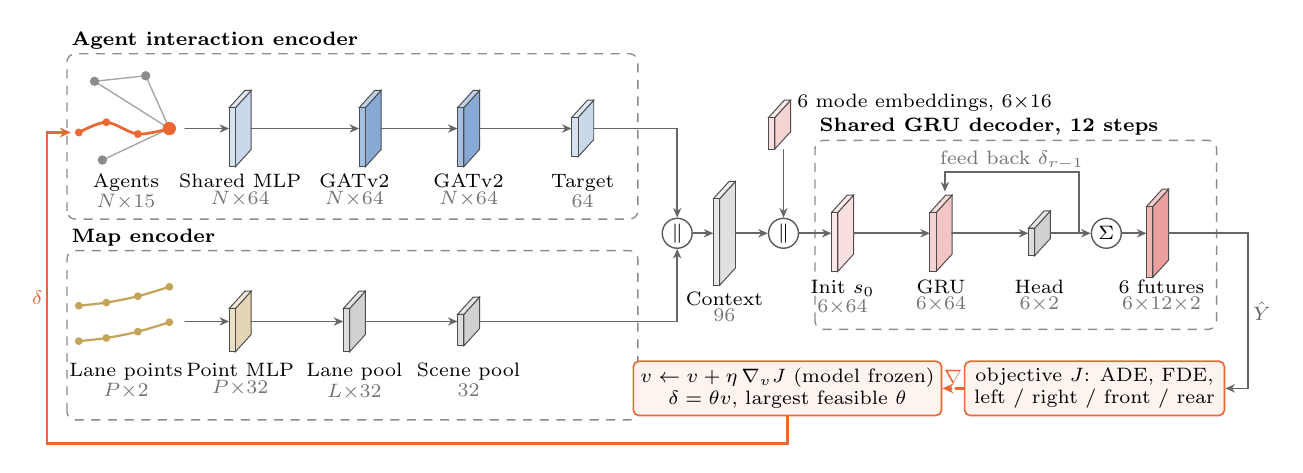
\begin{tikzpicture}[font=\scriptsize, line cap=round,
		frame/.style={draw=black!45, dashed, line width=0.5pt, rounded corners=3pt},
		ftitle/.style={font=\scriptsize\bfseries, anchor=south west, inner sep=1.5pt},
		lab/.style={align=center, anchor=north, inner sep=0.5pt},
		dim/.style={text=black!55, anchor=north, inner sep=0.5pt},
		flow/.style={-{Stealth[length=3.5pt, width=3pt]}, line width=0.6pt, black!60},
		atk/.style={-{Stealth[length=4pt, width=3.5pt]}, line width=0.8pt, attackC},
		op/.style={circle, draw=black!65, fill=white, line width=0.5pt, inner sep=0pt, minimum size=0.38cm},
		pgd/.style={draw=attackC, fill=attackC!8, line width=0.6pt, rounded corners=2pt, align=center, inner sep=2.5pt},
		gnode/.style={circle, fill, inner sep=1.2pt}]
	% ---------------- agent interaction encoder
	\draw[frame] (0, 2.6) rectangle (7.25, 4.7);
	\node[ftitle] at (0, 4.7) {Agent interaction encoder};
	% target with its observed past (orange: the only input the attacker changes) among real neighbours (grey)
	\foreach \a/\b in {0.35/4.35, 1.0/4.42, 0.45/3.35} \draw[black!35, line width=0.5pt] (1.3, 3.75) -- (\a, \b);
	\draw[black!35, line width=0.5pt] (0.35, 4.35) -- (1.0, 4.42);
	\foreach \a/\b in {0.35/4.35, 1.0/4.42, 0.45/3.35} \node[gnode, black!45] at (\a, \b) {};
	\draw[attackC, line width=1pt] plot[smooth] coordinates {(0.15, 3.7) (0.5, 3.83) (0.9, 3.68) (1.3, 3.75)};
	\foreach \a/\b in {0.15/3.7, 0.5/3.83, 0.9/3.68} \node[gnode, attackC, inner sep=1pt] at (\a, \b) {};
	\node[gnode, attackC, inner sep=1.7pt] at (1.3, 3.75) {};
	\node[lab] (L) at (0.75, 3.2) {Agents};
	\node[dim] at (L.south) {$N{\times}15$};
	\slab{mlp}{2.1}{3.75}{0.75}{cleanC!25}
	\slab{gat1}{3.75}{3.75}{0.75}{cleanC!55}
	\slab{gat2}{5.0}{3.75}{0.75}{cleanC!55}
	\slab{tgt}{6.45}{3.75}{0.5}{cleanC!25}
	\draw[flow] (1.5, 3.75) -- (mlp-in);
	\draw[flow] (mlp-out) -- (gat1-in);
	\draw[flow] (gat1-out) -- (gat2-in);
	\draw[flow] (gat2-out) -- (tgt-in);
	\foreach \x/\n/\d in {2.2/Shared MLP/N{\times}64, 3.65/GATv2/N{\times}64, 5.1/GATv2/N{\times}64, 6.55/Target/64} {
		\node[lab] (L) at (\x, 3.2) {\n};
		\node[dim] at (L.south) {$\d$};
	}
	% ---------------- map encoder
	\draw[frame] (0, 0.05) rectangle (7.25, 2.2);
	\node[ftitle] at (0, 2.2) {Map encoder};
	\foreach \y in {1.05, 1.5} {
		\draw[laneC, line width=0.8pt] plot[smooth] coordinates {(0.15, \y) (0.5, {\y+0.04}) (0.9, {\y+0.12}) (1.3, {\y+0.24})};
		\foreach \x/\d in {0.15/0, 0.5/0.04, 0.9/0.12, 1.3/0.24} \node[gnode, laneC, inner sep=1pt] at (\x, {\y+\d}) {};
	}
	\slab{pmlp}{2.1}{1.3}{0.55}{laneC!45}
	\slab{lpool}{3.55}{1.3}{0.55}{black!18}
	\slab{spool}{5.0}{1.3}{0.4}{black!18}
	\draw[flow] (1.5, 1.3) -- (pmlp-in);
	\draw[flow] (pmlp-out) -- (lpool-in);
	\draw[flow] (lpool-out) -- (spool-in);
	\foreach \x/\n/\d in {0.75/Lane points/P{\times}2, 2.2/Point MLP/P{\times}32, 3.65/Lane pool/L{\times}32, 5.1/Scene pool/32} {
		\node[lab] (L) at (\x, 0.8) {\n};
		\node[dim] at (L.south) {$\d$};
	}
	% ---------------- context and candidate embeddings
	\node[op] (cat1) at (7.75, 2.42) {$\Vert$};
	\draw[flow] (tgt-out) -| (cat1.north);
	\draw[flow] (spool-out) -| (cat1.south);
	\slab{ctx}{8.25}{2.42}{1.1}{black!12}
	\draw[flow] (cat1.east) -- (ctx-in);
	\node[lab] (L) at (8.35, 1.7) {Context};
	\node[dim] at (L.south) {96};
	\node[op] (cat2) at (9.1, 2.42) {$\Vert$};
	\draw[flow] (ctx-out) -- (cat2.west);
	\slab{modes}{8.95}{3.8}{0.4}{predC!20}
	\draw[flow] (9.1, 3.48) -- (cat2.north);
	\node[lab, anchor=south west] at (9.25, 3.95) {6 mode embeddings, $6{\times}16$};
	% ---------------- shared GRU decoder
	\draw[frame] (9.5, 1.2) rectangle (14.6, 3.6);
	\node[ftitle] at (9.5, 3.6) {Shared GRU decoder, 12 steps};
	\slab{h0}{9.75}{2.42}{0.75}{predC!15}
	\slab{gru}{11.0}{2.42}{0.75}{predC!28}
	\slab{head}{12.25}{2.42}{0.35}{black!18}
	\node[op] (sum) at (13.2, 2.42) {$\Sigma$};
	\slab{fut}{13.75}{2.42}{0.9}{predC!45}
	\draw[flow] (cat2.east) -- (h0-in);
	\draw[flow] (h0-out) -- (gru-in);
	\draw[flow] (gru-out) -- (head-in);
	\draw[flow] (head-out) -- (sum.west);
	\draw[flow] (sum.east) -- (fut-in);
	\draw[flow] (12.85, 2.42) -- (12.85, 3.2) -| (11.15, 2.95);
	\node[dim, anchor=south] at (12.0, 3.2) {feed back $\delta_{r-1}$};
	\foreach \x/\n/\d in {9.85/Init $s_0$/6{\times}64, 11.1/GRU/6{\times}64, 12.35/Head/6{\times}2, 13.9/6 futures/6{\times}12{\times}2} {
		\node[lab] (L) at (\x, 1.85) {\n};
		\node[dim] at (L.south) {$\d$};
	}
	% ---------------- PGD loop: objective -> gradient -> feasibility scaling -> target's past
	\node[pgd, minimum width=3.3cm] (goal) at (13.05, 0.45) {objective $J$: ADE, FDE,\\left / right / front / rear};
	\node[pgd, minimum width=3.2cm] (ascend) at (9.15, 0.45) {$v \leftarrow v + \eta\,\nabla_{v} J$ (model frozen)\\$\delta = \theta v$, largest feasible $\theta$};
	\draw[flow] (fut-out) -- (15.0, 2.42) |- node[pos=0.25, right, inner sep=1.5pt] {$\hat{Y}$} (goal.east);
	\draw[atk, dash pattern=on 3pt off 1.5pt] (goal) -- node[above, inner sep=1.5pt] {$\nabla$} (ascend);
	\draw[atk] (ascend.south) |- (-0.25, -0.25) |- (0.05, 3.7);
	\node[attackC, anchor=east, inner sep=1.5pt] at (-0.25, 1.6) {$\delta$};
\end{tikzpicture}

\caption{Final predictor with tensor sizes, and the attack. The attacker changes only the target's five observed points (orange); PGD ascends the objective through the frozen model and scales $\delta$ down until it is physically feasible.}
\label{fig:architecture}
\end{figure*}

\subsection{Trajectory prediction}
Most learned predictors pair an encoder of past motion, interactions and map with a decoder of future positions or their distribution. Recurrent models treat trajectories as time series: Social LSTM~\cite{alahi2016social} pools neighbouring LSTM states, and Trajectron++~\cite{salzmann2020trajectron} adds per-type edge LSTMs fused by attention and a conditional VAE decoder with dynamics integration. Rasterised methods such as MultiPath~\cite{chai2019multipath} and CoverNet~\cite{phanminh2020covernet} apply CNNs to bird's-eye-view images of map and histories, at the cost of discretisation. Vectorised methods avoid this: VectorNet~\cite{gao2020vectornet} encodes trajectories and lanes as polylines with a PointNet-like~\cite{qi2017pointnet} subgraph and lets all polylines interact through self-attention. Transformers such as MTR~\cite{shi2022mtr} now lead the benchmarks with similar vectorised scene representations.

\subsection{Adversarial robustness}
Small, crafted input perturbations can fool deep networks~\cite{goodfellow2015explaining}; PGD~\cite{madry2018pgd} finds them by iterated gradient ascent within a constraint set. Zhang et al.~\cite{zhang2022adversarial} first attacked trajectory prediction: the attacker drives a crafted trajectory within physical bounds on speed, acceleration and jerk, found by white-box PGD on the prediction error or its deviation in one direction. Across three models and three datasets, the worst-case error depended mostly on the target's own trajectory, and map input improved robustness.

\textit{Our approach.} We extend the attack of~\cite{zhang2022adversarial} to multimodal prediction. The predictor follows the vectorised paradigm in compact form: agents form a GATv2~\cite{brody2022gatv2} graph, and lanes are point sets, the PointNet special case of VectorNet's subgraph, fused late as one vector rather than joining the interaction graph.

\section{Method}
\subsection{Problem formulation and data}
Let $p_t\in\mathbb{R}^2$ be the target's position at step $t$, with $t=0$ the current time. At 2\,Hz the model observes $X=[p_{-4},\ldots,p_0]$ (2\,s) and predicts $K=6$ candidates $\hat{Y}^{(k)}=[\hat p^{(k)}_1,\ldots,\hat p^{(k)}_{12}]$ (6\,s), in a target-centred frame with $p_0=(0,0)$ and the current heading along $+x$. We use the nuScenes prediction split~\cite{caesar2020nuscenes}: the official train, train-val and val sets serve as our training (25{,}711 samples), validation (6{,}685) and test (7{,}242) sets. Each sample includes all vehicles and pedestrians within 35\,m (chosen by a sweep over 20/35/50\,m) that have a complete 2\,s history, and all lane centrelines intersecting a 100\,m$\times$100\,m box around the target, sampled every 1\,m.

\subsection{Model}
Fig.~\ref{fig:architecture} shows the architecture. \textit{History encoder.} Each agent $j$ is a node with features $x_j=[\mathrm{vec}(X_j);a_j]\in\mathbb{R}^{15}$, its five past positions and a five-class category one-hot $a_j$, embedded by a shared layer $h^{(0)}_j=\mathrm{ReLU}(W_h x_j+b_h)\in\mathbb{R}^{64}$. With five fixed-length points, a linear layer can represent velocity and acceleration, so we use no recurrent encoder.

\textit{Interaction encoder.} All nodes are connected by directed edges $j\to i$ with features $e_{ji}=[p^0_i-p^0_j;\,\lVert p^0_i-p^0_j\rVert]$ from current positions. Two GATv2 layers~\cite{brody2022gatv2} update the embeddings,
\begin{equation}
h^{(l+1)}_i=\mathrm{ReLU}\Big(\sum_{j\in\mathcal{N}(i)\cup\{i\}}\alpha^{(l)}_{ij}\,\Theta^{(l)}_t h^{(l)}_j\Big),
\end{equation}
where $\alpha_{ij}=\mathrm{softmax}_j\big(a^\top\mathrm{LeakyReLU}(\Theta_s h_i+\Theta_t h_j+\Theta_e e_{ji})\big)$. Edge features thus weight the messages but do not enter them. We keep the target's final embedding $h_T\in\mathbb{R}^{64}$.

\textit{Map encoder.} A shared two-layer MLP $\phi:\mathbb{R}^2\to\mathbb{R}^{32}$ embeds every lane point $q_{\ell,r}$, followed by max pooling within each lane and then across lanes: $u_\ell=\max_r\phi(q_{\ell,r})$, $m=\max_\ell u_\ell$. The context is $c=[h_T;m]\in\mathbb{R}^{96}$.

\textit{Decoder.} Each candidate $k$ has a learned embedding $z_k\in\mathbb{R}^{16}$ that initialises a GRU with hidden size 64, $s^{(k)}_0=\tanh(W_0[c;z_k])$. The GRU is fed its previous displacement (zero at the first step), $s^{(k)}_r=\mathrm{GRU}(\delta^{(k)}_{r-1},s^{(k)}_{r-1})$, $\delta^{(k)}_r=W_\delta s^{(k)}_r$, and positions are cumulative sums $\hat p^{(k)}_r=\sum_{\tau\le r}\delta^{(k)}_\tau$. Weights are shared across candidates.

\textit{Training.} We minimise the best-of-$K$ ADE, $\mathcal{L}=\min_k\frac{1}{12}\sum_r\lVert\hat p^{(k)}_r-p_r\rVert_2$, with Adam (learning rate $10^{-3}$, batch 64), keep the best validation checkpoint, and train every model with seeds 42, 123 and 2026. To isolate components we compare constant velocity (CV), a target-only MLP (no neighbours), a single-mode GATv2, a six-mode GATv2 with a one-shot MLP decoder, the same with the lane map, and the final model; the two map-aware models were trained for 60 epochs, the others for 30.

\subsection{Adversarial attack}
\begin{figure*}[t]
\centering
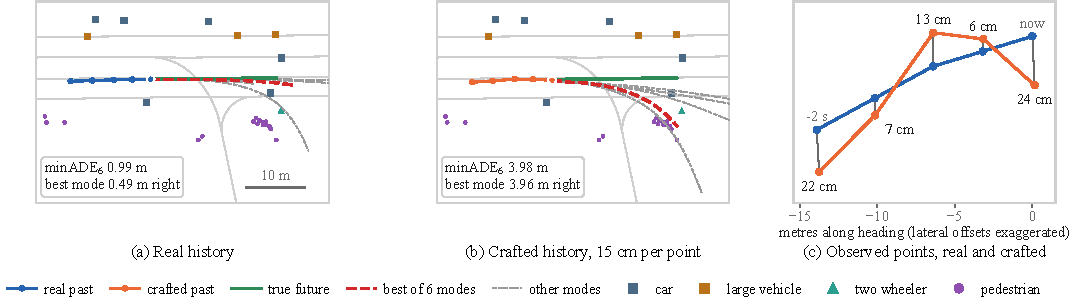
\includegraphics[width=\textwidth]{figures/attack_example.pdf}
\caption{Right attack on the final model (seed 42, nuScenes scene-0241; chosen for clarity, not representative): 15\,cm per point moves the best candidate 3.96\,m right.}
\label{fig:example}
\end{figure*}

\textit{Threat model.} As in~\cite{zhang2022adversarial}, an attacker drives the target vehicle along a crafted history $\tilde X=X+\delta$, $\delta\in\mathbb{R}^{5\times2}$, knowing the model and the ground-truth future (white-box, single frame). Neighbours and lanes stay fixed in world coordinates; because our frame is target-centred, a shift $d=\delta_0$ of the current position moves all agent and lane positions by $-d$, edge features are recomputed differentiably, and predictions are shifted back before evaluation.

\textit{Constraints.} Each point moves at most 1\,m, and the perturbed history, joined with the first three ground-truth future points, must satisfy the nuScenes bounds of~\cite{zhang2022adversarial} on speed, longitudinal and lateral acceleration, and jerk. A candidate $v$ is scaled by the largest $\theta\in\{1.00,0.99,\ldots,0.02\}$ that makes $\theta v$ feasible ($\theta=0$ if none).

\textit{Objectives.} One attack is run per objective $J$: the overall errors $\min_k\frac{1}{12}\sum_r\lVert\hat p^{(k)}_r-p_r\rVert^2$ and $\min_k\lVert\hat p^{(k)}_{12}-p_{12}\rVert^2$, and the signed deviation of the min-ADE candidate $k^*$ towards the left, right, front or rear,
\begin{equation}
D=\frac{1}{12}\sum_{r=1}^{12}\big(\hat p^{(k^*)}_r-p_r\big)^\top R_r,
\end{equation}
where $R_r$ is a unit vector along (front, rear) or perpendicular to (left, right) the ground-truth motion direction $p_r-p_{r-1}$.

\textit{Optimisation.} We run 10 random restarts of 100 plain gradient steps on $-J(\theta v)$ from $v\sim U[-1,1]$\,m (learning rate 0.01 for the overall errors, 0.1 for the directions; $\theta$ fixed within a step) and keep the best perturbation, with $\delta=0$ as the reference. As a control, smooth random perturbations (an offset plus a linear drift) of the attack's mean size, with the same scaling, are averaged over 20 draws.

\subsection{Metrics}
We report \minade{}, \minfde{} (candidates chosen independently), $D$ and, as in~\cite{zhang2022adversarial}, the share of samples deviating more than 1.85\,m (half a lane) in the attacked direction, a proxy for real-world impact; single-mode models use their only prediction. Every model is attacked on the same 500 random validation samples, and values are means over seeds. We also group samples by ground-truth motion (slow if the endpoint is within 5\,m, otherwise straight or turning at a 15$^\circ$ endpoint angle) and by current speed.

\subsection{Implementation statement}\label{sec:impl}
The predictor (data pipeline, models, training and the test results in Section~\ref{sec:accuracy}) was developed mainly by the other pair of our project group. We contributed reproducibility and optimisation work: seed control, pinned environments, checkpoint manifests, repository-relative paths, a fully connected graph with distance features instead of a pairwise edge cutoff, and the automated neighbour-radius sweep. All attacked checkpoints are used unchanged. We wrote the attack and evaluation code: the differentiable re-centring of agents and lanes, the multimodal objectives and metrics, the random control, the CV baseline, and all analyses in Sections~\ref{sec:vulnerable}--\ref{sec:why}. From the code of~\cite{zhang2022adversarial} we adapted the physical bounds, the $\theta$-scaling search and the PGD settings; following their paper rather than their code, our feasibility check includes the next three ground-truth points, and we report the feasible share of clean histories (84\%). Libraries: PyTorch, PyTorch Geometric, the nuScenes devkit and Matplotlib.

\begin{table}[t]
\centering
\caption{Results on 500 validation samples (mean of three seeds). Shares deviate over 1.85\,m in the attacked direction; last column: error added per metre of perturbation (ADE attack). $K{=}1$ for the first three models.}
\label{tab:ladder}
\footnotesize
\setlength{\tabcolsep}{3pt}
\begin{tabular}{@{}lcccc@{}}
\toprule
& minADE$_K$ (m) & Lateral (\%) & Longit.\ (\%) & m per m \\
Model & clean$\to$att. & clean$\to$att. & clean$\to$att. & \\
\midrule
CV & 4.46$\to$8.00 & 11$\to$37 & 31$\to$72 & 20.8 \\
Target-only MLP & 3.63$\to$8.52 & 10$\to$59 & 29$\to$79 & 23.6 \\
GATv2 & 3.54$\to$8.10 & 10$\to$53 & 29$\to$77 & 21.4 \\
GATv2, $K{=}6$ & 1.71$\to$3.46 & \phantom{0}6$\to$38 & \phantom{0}8$\to$68 & \phantom{0}9.2 \\
\quad + lane map & 1.49$\to$2.82 & \phantom{0}3$\to$21 & \phantom{0}5$\to$49 & \phantom{0}7.0 \\
\quad + GRU (final) & 1.46$\to$2.82 & \phantom{0}3$\to$17 & \phantom{0}6$\to$49 & \phantom{0}7.3 \\
\bottomrule
\end{tabular}
\end{table}

\begin{table}[t]
\centering
\caption{Final model by ground-truth motion and current speed; columns and all-sample values in Table~\ref{tab:ladder}.}
\label{tab:strata}
\footnotesize
\setlength{\tabcolsep}{3pt}
\begin{tabular}{@{}lrccc@{}}
\toprule
& & \minade{} (m) & Lateral (\%) & Longit.\ (\%) \\
Group & $n$ & clean$\to$att. & clean$\to$att. & clean$\to$att. \\
\midrule
Slow ($<$5\,m in 6\,s) & 21 & 0.61$\to$3.29 & \phantom{0}0$\to$\phantom{0}6 & \phantom{0}0$\to$29 \\
Straight ($<$15$^\circ$) & 376 & 1.25$\to$2.51 & \phantom{0}1$\to$12 & \phantom{0}4$\to$50 \\
Turning ($\ge$15$^\circ$) & 103 & 2.41$\to$3.84 & 11$\to$40 & 14$\to$52 \\
\midrule
Speed $<$2\,m/s & 108 & 1.36$\to$3.10 & \phantom{0}2$\to$19 & \phantom{0}7$\to$45 \\
Speed 2--8\,m/s & 305 & 1.50$\to$2.80 & \phantom{0}4$\to$18 & \phantom{0}6$\to$54 \\
Speed $\ge$8\,m/s & 87 & 1.46$\to$2.52 & \phantom{0}2$\to$11 & \phantom{0}5$\to$37 \\
\bottomrule
\end{tabular}
\end{table}

\section{Results and Discussion}
\subsection{Prediction accuracy}\label{sec:accuracy}
On the test split, the final model reaches \minade{} $1.474\pm0.016$\,m and \minfde{} $2.931\pm0.044$\,m (mean $\pm$ std over seeds), 3.8\% and 6.1\% better than an otherwise identical one-shot MLP decoder ($1.533$ and $3.121$\,m) and 11.6\% and 18.1\% better on 30--60$^\circ$ turns.

\subsection{How vulnerable is the final model?}\label{sec:vulnerable}
Under attack, \minade{} rises from 1.46 to 2.82\,m ($\times$1.93) and \minfde{} from 3.03 to 6.01\,m ($\times$1.99), and 33\% of predictions deviate more than half a lane in the attacked direction (4\% clean), with a mean perturbation of only 0.18\,m per point (Figs.~\ref{fig:example} and~\ref{fig:fragility}a). Same-size random perturbations change \minade{} by 0.02\,m and leave the half-lane share at 4\%, so the direction of the perturbation matters, not its size. The 16\% of clean histories that violate the bounds mostly stay unperturbed; without them the share is 35--38\%. Zhang et al.\ report higher averages ($+$167\% ADE, $+$150\% FDE, 62\%; ours: $+$93\%, $+$99\%, 33\%) for other models and data.

\subsection{Which components add robustness?}
Longitudinal attacks succeed more often than lateral ones for every model (Table~\ref{tab:ladder}), as a slightly faster or slower history is extrapolated over 6\,s. Only the lane map has a clear effect: added to the six-mode GATv2, it lowers lateral success from 38\% to 21\%, longitudinal success from 68\% to 49\%, and the attacked \minade{} from 3.46 to 2.82\,m, in line with the 31\% reduction for Trajectron++ in~\cite{zhang2022adversarial}; lanes cannot be moved by the attacker. Neighbours barely help (single-mode GATv2 vs.\ target-only MLP: 53\% vs.\ 59\% lateral, 77\% vs.\ 79\% longitudinal), and the GRU decoder lowers lateral success only from 21\% to 17\%. Six-mode models look more robust partly because best-of-six needs only one close candidate. The map models trained twice as long, but in a single-seed check this changed clean \minade{} by only 0.01\,m.

\subsection{When does the attack succeed?}
Lateral attacks succeed on 40\% of turning but 12\% of straight samples (Table~\ref{tab:strata}); turning samples are already harder (clean \minade{} 2.41 vs.\ 1.25\,m; 11\% vs.\ 1\% beyond half a lane without attack). Slow targets show the largest relative increase ($\times$5.4), as a crafted history fakes motion that the model extrapolates, but only 21 samples are slow. Fast targets ($\ge$8\,m/s) are pushed past half a lane least often.

\begin{figure}[t]
\centering
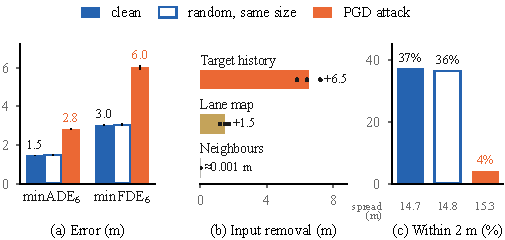
\includegraphics[width=\columnwidth]{figures/fragility.pdf}
\caption{(a) Errors (mean $\pm$ std over seeds). (b) \minade{} added when an input is removed, full validation set (dots: seeds). (c) Samples with a candidate within 2\,m at every step, ADE attack; endpoint spread below.}
\label{fig:fragility}
\end{figure}

\subsection{Why is the model easy to fool?}\label{sec:why}
Short history, long horizon. Velocity is inferred from five points, so a small shift grows over 12 steps: even CV adds 20.8\,m of error per metre of perturbation, the final model 7.3\,m (Table~\ref{tab:ladder}).

Reliance on what the attacker controls (Fig.~\ref{fig:fragility}b). Replacing the target's history by its current position raises \minade{} by 5.8--7.2\,m, removing the map by 1.2--1.7\,m, and removing all neighbours by at most 0.001\,m. Removal creates inputs unlike the training data, so these are not precise causal importances, but the negligible neighbour effect shows that the models make little use of neighbours: in two of three seeds, neighbours put almost all first-layer attention on the target and carry a copy of its encoding.

Candidates move together (Fig.~\ref{fig:fragility}c). All six are decoded from one context: under the ADE attack their spread changes by about 5\%, yet samples with a candidate within 2\,m of the truth fall from 37\% to 4\%. The whole fan shifts, so multimodality offers little protection.

\section{Conclusions and Future Work}
We evaluated the robustness of a map-aware multimodal GNN predictor to adversarial driving scenarios. A shift of just 18\,cm per observed point doubles prediction errors and pushes a third of forecasts more than half a lane off, most often during turning manoeuvres, whereas equivalent random noise causes no measurable disruption. Because an adversary cannot manipulate the road layout, high-definition lane maps serve as the primary buffer against these attacks. In contrast, modelled agent interactions offer virtually no defensive benefit, as the network largely overlooks the neighbours. Ultimately, this vulnerability exposes a fundamental blind spot: the model fails to cross-validate a target vehicle's past trajectory against its surroundings.

Our evaluation has several limitations, including its white-box access, single-frame attack setup, a sample size of 500 validation samples, the 1.85\,m displacement proxy, and kinematic bounds that do not guarantee drivable trajectories.

Future work: We aim to investigate architectures that genuinely leverage neighbouring agents such as Trajectron++~\cite{salzmann2020trajectron} using temporal relative-motion edge features and lanes fused through attention as in VectorNet~\cite{gao2020vectornet}, adversarial training, and attacks that propagate through the graph.

\bibliographystyle{IEEEtran}
\bibliography{refs}

\end{document}
